\documentclass{standalone}
\usepackage{tikz}
\usetikzlibrary{patterns, positioning}


\begin{document}
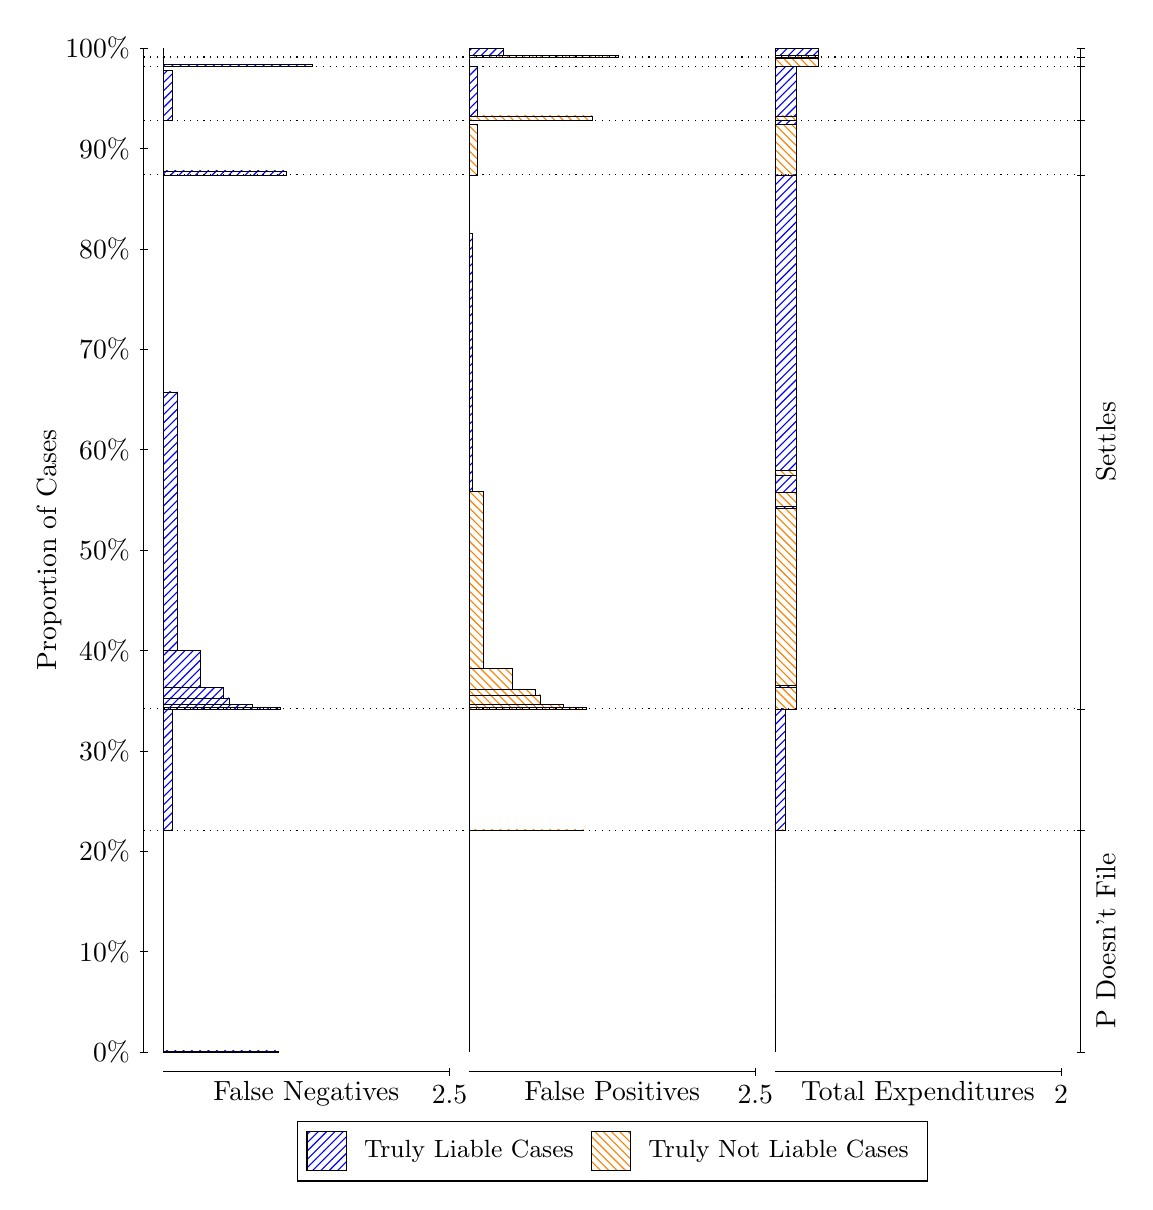
\begin{tikzpicture}
\draw[black, very thin] (1.5,1.75) -- (1.5,14.5);
\node[rotate=90, text=black, anchor=center] at (0.3, 8.125) {Proportion of Cases};
\draw[black, very thin] (1.45,1.75) -- (1.55,1.75);
\node[text=black, anchor=east] at (1.45, 1.75) {0\%};
\draw[black, very thin] (1.45,3.025) -- (1.55,3.025);
\node[text=black, anchor=east] at (1.45, 3.025) {10\%};
\draw[black, very thin] (1.45,4.3) -- (1.55,4.3);
\node[text=black, anchor=east] at (1.45, 4.3) {20\%};
\draw[black, very thin] (1.45,5.575) -- (1.55,5.575);
\node[text=black, anchor=east] at (1.45, 5.575) {30\%};
\draw[black, very thin] (1.45,6.85) -- (1.55,6.85);
\node[text=black, anchor=east] at (1.45, 6.85) {40\%};
\draw[black, very thin] (1.45,8.125) -- (1.55,8.125);
\node[text=black, anchor=east] at (1.45, 8.125) {50\%};
\draw[black, very thin] (1.45,9.4) -- (1.55,9.4);
\node[text=black, anchor=east] at (1.45, 9.4) {60\%};
\draw[black, very thin] (1.45,10.675) -- (1.55,10.675);
\node[text=black, anchor=east] at (1.45, 10.675) {70\%};
\draw[black, very thin] (1.45,11.95) -- (1.55,11.95);
\node[text=black, anchor=east] at (1.45, 11.95) {80\%};
\draw[black, very thin] (1.45,13.225) -- (1.55,13.225);
\node[text=black, anchor=east] at (1.45, 13.225) {90\%};
\draw[black, very thin] (1.45,14.5) -- (1.55,14.5);
\node[text=black, anchor=east] at (1.45, 14.5) {100\%};

\draw[black, very thin] (13.4,1.75) -- (13.4,14.5);
\draw[black, very thin] (13.35,1.75) -- (13.45,1.75);
\node[anchor=west] at (13.35, 1.75) {};
\draw[black, very thin] (13.35,4.5683) -- (13.45,4.5683);
\node[anchor=west] at (13.35, 4.5683) {};
\draw[black, very thin] (13.35,6.1073) -- (13.45,6.1073);
\node[anchor=west] at (13.35, 6.1073) {};
\draw[black, very thin] (13.35,12.89) -- (13.45,12.89);
\node[anchor=west] at (13.35, 12.89) {};
\draw[black, very thin] (13.35,13.581) -- (13.45,13.581);
\node[anchor=west] at (13.35, 13.581) {};
\draw[black, very thin] (13.35,14.271) -- (13.45,14.271);
\node[anchor=west] at (13.35, 14.271) {};
\draw[black, very thin] (13.35,14.386) -- (13.45,14.386);
\node[anchor=west] at (13.35, 14.386) {};
\draw[black, very thin] (13.35,14.5) -- (13.45,14.5);
\node[anchor=west] at (13.35, 14.5) {};

\draw[black, very thin, pattern color=blue, pattern=north east lines] (1.75,1.75) rectangle (3.2033,1.7649);
\draw[black, very thin, pattern color=orange, pattern=north west lines] (1.75,1.7649) rectangle (1.75,4.5683);
\draw[black, very thin, pattern color=blue, pattern=north east lines] (1.75,4.5683) rectangle (1.859,6.1039);
\draw[black, very thin, pattern color=orange, pattern=north west lines] (1.75,6.1039) rectangle (1.75,6.1073);
\draw[black, very thin, pattern color=blue, pattern=north east lines] (1.75,6.1073) rectangle (3.2397,6.1278);
\draw[black, very thin, pattern color=blue, pattern=north east lines] (1.75,6.1278) rectangle (2.8763,6.1613);
\draw[black, very thin, pattern color=blue, pattern=north east lines] (1.75,6.1613) rectangle (2.5857,6.2469);
\draw[black, very thin, pattern color=blue, pattern=north east lines] (1.75,6.2469) rectangle (2.513,6.3761);
\draw[black, very thin, pattern color=blue, pattern=north east lines] (1.75,6.3761) rectangle (2.2223,6.8518);
\draw[black, very thin, pattern color=blue, pattern=north east lines] (1.75,6.8518) rectangle (1.9317,10.133);
\draw[black, very thin, pattern color=orange, pattern=north west lines] (1.75,10.133) rectangle (1.75,12.89);
\draw[black, very thin, pattern color=blue, pattern=north east lines] (1.75,12.89) rectangle (3.3123,12.94);
\draw[black, very thin, pattern color=orange, pattern=north west lines] (1.75,12.94) rectangle (1.75,13.581);
\draw[black, very thin, pattern color=blue, pattern=north east lines] (1.75,13.581) rectangle (1.859,14.215);
\draw[black, very thin, pattern color=orange, pattern=north west lines] (1.75,14.215) rectangle (1.75,14.271);
\draw[black, very thin, pattern color=blue, pattern=north east lines] (1.75,14.271) rectangle (3.6393,14.289);
\draw[black, very thin, pattern color=orange, pattern=north west lines] (1.75,14.289) rectangle (1.75,14.386);
\draw[black, very thin, pattern color=orange, pattern=north west lines] (1.75,14.386) rectangle (1.75,14.403);
\draw[black, very thin, pattern color=blue, pattern=north east lines] (1.75,14.403) rectangle (1.75,14.5);
\draw[black, very thin, pattern color=orange, pattern=north west lines] (5.6333,1.75) rectangle (5.6333,4.5534);
\draw[black, very thin, pattern color=blue, pattern=north east lines] (5.6333,4.5534) rectangle (5.6333,4.5683);
\draw[black, very thin, pattern color=orange, pattern=north west lines] (5.6333,4.5683) rectangle (7.0867,4.5716);
\draw[black, very thin, pattern color=blue, pattern=north east lines] (5.6333,4.5716) rectangle (5.6333,6.1073);
\draw[black, very thin, pattern color=orange, pattern=north west lines] (5.6333,6.1073) rectangle (7.123,6.125);
\draw[black, very thin, pattern color=orange, pattern=north west lines] (5.6333,6.125) rectangle (6.8323,6.1662);
\draw[black, very thin, pattern color=orange, pattern=north west lines] (5.6333,6.1662) rectangle (6.5417,6.2839);
\draw[black, very thin, pattern color=orange, pattern=north west lines] (5.6333,6.2839) rectangle (6.469,6.3518);
\draw[black, very thin, pattern color=orange, pattern=north west lines] (5.6333,6.3518) rectangle (6.1783,6.6213);
\draw[black, very thin, pattern color=orange, pattern=north west lines] (5.6333,6.6213) rectangle (5.815,8.8648);
\draw[black, very thin, pattern color=blue, pattern=north east lines] (5.6333,8.8648) rectangle (5.6697,12.146);
\draw[black, very thin, pattern color=blue, pattern=north east lines] (5.6333,12.146) rectangle (5.6333,12.89);
\draw[black, very thin, pattern color=orange, pattern=north west lines] (5.6333,12.89) rectangle (5.7423,13.53);
\draw[black, very thin, pattern color=blue, pattern=north east lines] (5.6333,13.53) rectangle (5.6333,13.581);
\draw[black, very thin, pattern color=orange, pattern=north west lines] (5.6333,13.581) rectangle (7.1957,13.637);
\draw[black, very thin, pattern color=blue, pattern=north east lines] (5.6333,13.637) rectangle (5.7423,14.271);
\draw[black, very thin, pattern color=orange, pattern=north west lines] (5.6333,14.271) rectangle (5.6333,14.368);
\draw[black, very thin, pattern color=blue, pattern=north east lines] (5.6333,14.368) rectangle (5.6333,14.386);
\draw[black, very thin, pattern color=orange, pattern=north west lines] (5.6333,14.386) rectangle (7.5227,14.403);
\draw[black, very thin, pattern color=blue, pattern=north east lines] (5.6333,14.403) rectangle (6.0693,14.5);
\draw[black, very thin, pattern color=orange, pattern=north west lines] (9.5167,1.75) rectangle (9.5167,4.5534);
\draw[black, very thin, pattern color=blue, pattern=north east lines] (9.5167,4.5534) rectangle (9.5167,4.5683);
\draw[black, very thin, pattern color=orange, pattern=north west lines] (9.5167,4.5683) rectangle (9.6529,4.5716);
\draw[black, very thin, pattern color=blue, pattern=north east lines] (9.5167,4.5716) rectangle (9.6529,6.1073);
\draw[black, very thin, pattern color=orange, pattern=north west lines] (9.5167,6.1073) rectangle (9.7892,6.3768);
\draw[black, very thin, pattern color=blue, pattern=north east lines] (9.5167,6.3768) rectangle (9.7892,6.4103);
\draw[black, very thin, pattern color=orange, pattern=north west lines] (9.5167,6.4103) rectangle (9.7892,8.6537);
\draw[black, very thin, pattern color=blue, pattern=north east lines] (9.5167,8.6537) rectangle (9.7892,8.6743);
\draw[black, very thin, pattern color=orange, pattern=north west lines] (9.5167,8.6743) rectangle (9.7892,8.8598);
\draw[black, very thin, pattern color=blue, pattern=north east lines] (9.5167,8.8598) rectangle (9.7892,9.0746);
\draw[black, very thin, pattern color=orange, pattern=north west lines] (9.5167,9.0746) rectangle (9.7892,9.1336);
\draw[black, very thin, pattern color=blue, pattern=north east lines] (9.5167,9.1336) rectangle (9.7892,12.89);
\draw[black, very thin, pattern color=orange, pattern=north west lines] (9.5167,12.89) rectangle (9.7892,13.53);
\draw[black, very thin, pattern color=blue, pattern=north east lines] (9.5167,13.53) rectangle (9.7892,13.581);
\draw[black, very thin, pattern color=orange, pattern=north west lines] (9.5167,13.581) rectangle (9.7892,13.637);
\draw[black, very thin, pattern color=blue, pattern=north east lines] (9.5167,13.637) rectangle (9.7892,14.271);
\draw[black, very thin, pattern color=orange, pattern=north west lines] (9.5167,14.271) rectangle (10.062,14.368);
\draw[black, very thin, pattern color=blue, pattern=north east lines] (9.5167,14.368) rectangle (10.062,14.386);
\draw[black, very thin, pattern color=orange, pattern=north west lines] (9.5167,14.386) rectangle (10.062,14.403);
\draw[black, very thin, pattern color=blue, pattern=north east lines] (9.5167,14.403) rectangle (10.062,14.5);
\draw[black, dotted] (1.5,4.5683) -- (13.4,4.5683);
\draw[black, dotted] (1.5,6.1073) -- (13.4,6.1073);
\draw[black, dotted] (1.5,12.89) -- (13.4,12.89);
\draw[black, dotted] (1.5,13.581) -- (13.4,13.581);
\draw[black, dotted] (1.5,14.271) -- (13.4,14.271);
\draw[black, dotted] (1.5,14.386) -- (13.4,14.386);
\draw[black, very thin] (1.75,1.5) -- (5.3833,1.5);
\node[text=black, anchor=north] at (3.5667, 1.5) {False Negatives};
\draw[black, very thin] (5.3833,1.45) -- (5.3833,1.55);
\node[text=black, anchor=north] at (5.3833, 1.45) {2.5};

\draw[black, very thin] (5.6333,1.5) -- (9.2667,1.5);
\node[text=black, anchor=north] at (7.45, 1.5) {False Positives};
\draw[black, very thin] (9.2667,1.45) -- (9.2667,1.55);
\node[text=black, anchor=north] at (9.2667, 1.45) {2.5};

\draw[black, very thin] (9.5167,1.5) -- (13.15,1.5);
\node[text=black, anchor=north] at (11.333, 1.5) {Total Expenditures};
\draw[black, very thin] (13.15,1.45) -- (13.15,1.55);
\node[text=black, anchor=north] at (13.15, 1.45) {2};

\node[text=black, centered, rotate=90] at (13.72, 3.1591) {P Doesn't File};

\node[text=black, centered, rotate=90] at (13.72, 9.4987) {Settles};





\draw (7.449999999999999,1.5) node[draw=none] (baseCoordinate) {};
\begin{scope}[align=center]
        \matrix[scale=0.5, draw=black, below=0.5cm of baseCoordinate, nodes={draw}, column sep=0.1cm]{
            \node[rectangle, draw, minimum width=0.5cm, minimum height=0.5cm, pattern color=blue, pattern=north east lines] {}; &
            \node[draw=none, font=\small, text=black] (B) {Truly Liable Cases}; &
            \node[rectangle, draw, minimum width=0.5cm, minimum height=0.5cm, pattern color=orange, pattern=north west lines] {}; &
            \node[draw=none, font=\small, text=black] (B) {Truly Not Liable Cases}; \\
            };
\end{scope}

\end{tikzpicture}
\end{document}